\documentclass{article}
\usepackage{v-problem}
\vgeometry

\begin{document}
\vtitle[ELECTROSTATICS]

\def\pn{11}
\def\book{Irodov}
\def\page{106}
\def\gdrive{Link}

\def\question{
A thin non-conducting ring of radius R has a linear charge density $\lambda=\lambda_0 \cos\phi$, where $\lambda_0$ is a constant, $\phi$ is the azimuthal angle. Find the magnitude of the electric field strength at the center of the ring.
}

\vspace*{\fill}
\begin{tikzpicture}
	\node[qnumber] (n) at (0, 0)[scale=2] {$\pn.$};
	\node[question] (q) [right=2mm of n.east] {\question};
	\tzline[divider]<-0.125, 0> (q.north west)(q.south west);
	\node[format] (f) at  (q.south east){[\book \quad \page]};
\end{tikzpicture}	
\vspace*{\fill}

\begin{center}
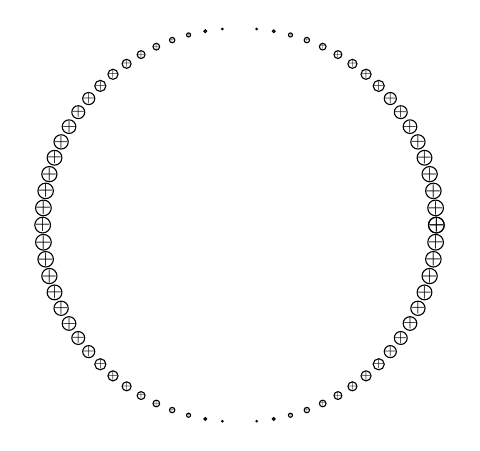
\begin{tikzpicture}
\def\R{2.5}
	\foreach \a in {0, 5, ..., 360}{
		\draw (\a:\R) circle[radius=0.1*cos(\a)];
		\node at (\a:\R)[scale=0.75*cos(\a)] {$+$};
	}
\end{tikzpicture}
\end{center}

\pagebreak

\vspace*{\fill}
\begin{center}
	\fbox{\qrcode[height=2cm]{\gdrive}}
\end{center}
\vspace*{\fill}

\end{document}
